\usetikzlibrary{automata,positioning}
\tikzstyle{edge} = [draw,thick,->]
\begin{center}
  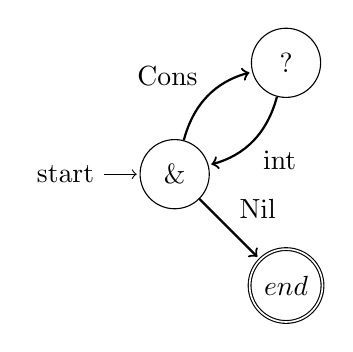
\begin{tikzpicture}[shorten >=1pt,node distance=2cm,on grid,auto] 
   \node[state,initial] (choice)   {$\&$}; 
   \node[state] (input) [above right=of choice] {$?$}; 
   \node[state,accepting] (end) [below right=of choice] {$end$}; 

   \path[edge] (choice) to[bend left] node {Cons} (input);
   \path[edge] (input) to[bend left] node {int} (choice);
   \path[edge] (choice) edge node {Nil} (end);
   
  \end{tikzpicture}
\end{center}

%%% Local Variables:
%%% mode: latex
%%% TeX-master: "cfst-inforum18"
%%% End: